\documentclass[aspectratio=169]{beamer}

\mode<presentation> {
	\usetheme{Madrid}
	\setbeamertemplate{navigation symbols}{}
}

% ---------- 页尾 ----------
\setbeamertemplate{footline}{
	\begin{beamercolorbox}[wd=\paperwidth,ht=2.5ex,dp=1.25ex]{footline}
		\usebeamerfont{footline}\hspace{0.2cm}\insertshortinstitute%
		\hfill\insertshorttitle\hfill%
		\insertframenumber/\inserttotalframenumber\hspace{0.2cm}%
	\end{beamercolorbox}
}
\setbeamercolor{footline}{fg=orchiddark,bg=orchidlight!30}

% ---------- 二月兰紫配色 ----------
\definecolor{orchidpurple}{RGB}{146,39,143}
\definecolor{orchiddark}{RGB}{115,30,112}
\definecolor{orchidlight}{RGB}{230,210,230}
\definecolor{orchidteal}{RGB}{0,128,128}
\definecolor{orchidteallight}{RGB}{214,235,235}
\definecolor{orchidgold}{RGB}{198,140,0}
\definecolor{orchidgoldlight}{RGB}{250,240,216}

\setbeamercolor{structure}{fg=orchidpurple}
\setbeamercolor{palette primary}{fg=white,bg=orchidpurple}
\setbeamercolor{palette secondary}{fg=white,bg=orchiddark}
\setbeamercolor{palette tertiary}{fg=white,bg=orchidpurple}
\setbeamercolor{palette quaternary}{fg=white,bg=orchiddark}
\setbeamercolor{titlelike}{fg=white,bg=orchidpurple}
\setbeamercolor{frametitle}{fg=white,bg=orchidpurple}
\setbeamercolor{block title}{fg=white,bg=orchidpurple}
\setbeamercolor{block body}{fg=black,bg=orchidlight!30}
\setbeamercolor{item}{fg=orchidpurple}
\setbeamercolor{section in toc}{fg=orchiddark}
\setbeamercolor{block title alerted}{fg=white,bg=orchidteal}
\setbeamercolor{block body alerted}{fg=black,bg=orchidteallight}
\setbeamercolor{block title example}{fg=white,bg=orchidgold}
\setbeamercolor{block body example}{fg=black,bg=orchidgoldlight}

\usepackage{graphicx}
\usepackage{booktabs}
\usepackage[UTF8,noindent]{ctexcap}
\usepackage[bookmarks=true]{hyperref}
\usepackage{amsmath,amssymb,bm}
\usepackage{tikz}
\usetikzlibrary{shapes.geometric,arrows,positioning}

% ---------- 快捷命令 ----------
\newcommand{\T}{^{\mathsf{T}}}
\newcommand{\R}{\mathbb{R}}
\newcommand{\mat}[1]{\bm{#1}}
\newcommand{\tbf}[1]{\textbf{#1}}

% ============================================================
%	以下为可修改区：标题 / 作者 / 单位 / 日期
% ============================================================

\title[063组分享]{《波浪能装置输出功率优化设计》赏析}
\author{魏舟}
\institute[南京理工大学]
{
	063组 \\
	\medskip
	\textit{wei\_zhou@njust.edu.cn}
}
\date{2026年8月}

% ============================================================
%	以下为正文示例，请按需替换
% ============================================================

\begin{document}

% ---------- 标题页 ----------
\begin{frame}
	\begin{center}
		\begin{beamercolorbox}[rounded=true,shadow=true,sep=8pt,center,wd=\textwidth]{title}
			\usebeamerfont{title}\inserttitle
		\end{beamercolorbox}
	\end{center}
	\vspace{0.5cm}
	\begin{columns}[c]
		\column{0.5\textwidth}
		\centering
		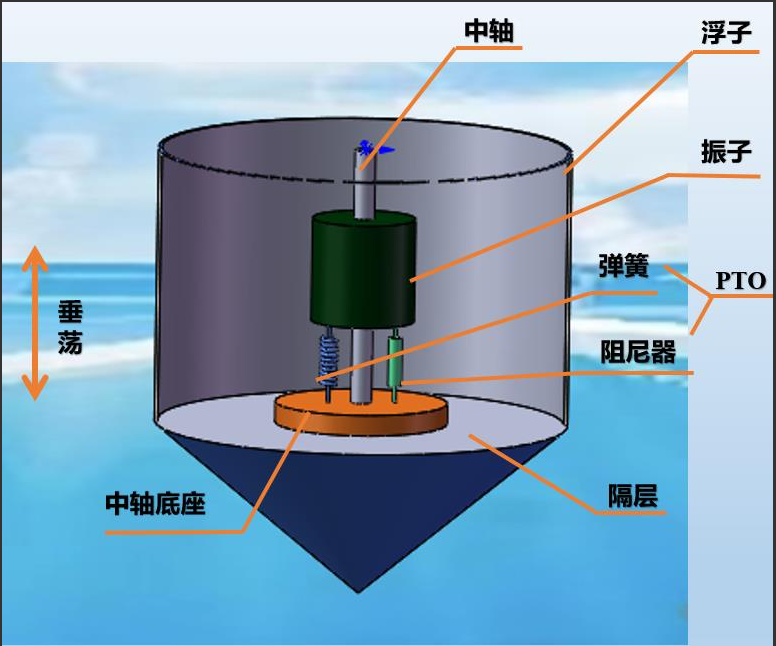
\includegraphics[width=0.9\textwidth]{Figure/波浪能装置示意图.png}

		\column{0.5\textwidth}
		\centering
		{\usebeamerfont{author}\usebeamercolor[fg]{author}\insertauthor}\\[0.4cm]
		{\usebeamerfont{institute}\usebeamercolor[fg]{institute}\insertinstitute}\\[0.4cm]
		{\usebeamerfont{date}\usebeamercolor[fg]{date}\insertdate}
	\end{columns}
\end{frame}

% ---------- 目录 ----------
\section*{目录}
\begin{frame}
	\frametitle{汇报提纲}
	\tableofcontents
\end{frame}


\section{文章结构}
\begin{frame}
	\frametitle{文章结构}
	\begin{center}
	\begin{tikzpicture}[
		box/.style={draw=orchidpurple, thick, rounded corners=3pt,
			minimum width=2.2cm, minimum height=1.2cm, align=center,
			fill=orchidlight!40},
		arrow/.style={-stealth, thick, orchidpurple}
	]
		\node[box] (a) at (0,0) {问题重述};
		\node[box] (b) at (4.8,0) {问题分析};
		\node[box] (c) at (9.6,0) {模型假设};
		\node[box] (d) at (9.6,-2.4) {模型的建立\\与求解};
		\node[box] (e) at (4.8,-2.4) {模型检验\\(分析)};
		\node[box, fill=orchidpurple, text=white] (f) at (0,-2.4) {总结};

		\draw[arrow] (a.east) -- (b.west);
		\draw[arrow] (b.east) -- (c.west);
		\draw[arrow] (c.south) -- (d.north);
		\draw[arrow] (d.west) -- (e.east);
		\draw[arrow] (e.west) -- (f.east);
	\end{tikzpicture}
	\end{center}
	这篇文章的结构，是一个非常经典的数模论文的结构，涵盖了从问题重述到模型建立与求解，再到模型检验和总结的完整流程。也和我们数学建模课程中学习到的一模一样。
\end{frame}

\section{标题分析}
\begin{frame}
	\frametitle{标题分析：一般AI撰写的标题}
	\small
	\begin{columns}[T]
		\column{0.58\textwidth}
		\begin{block}{标题 1}
			《基于随机优化与动态规划的航空舱位分配与动态定价策略研究》
		\end{block}
		\begin{block}{标题 2}
			《基于嵌入式 MCU 的铝制工件表面缺陷检测系统》
		\end{block}
		\begin{block}{标题 3}
			《基于组合赋权-TOPSIS 与 Huff 引力模型的城市商圈消费活力评价与首店选址研究》
		\end{block}

		\column{0.42\textwidth}
		\begin{block}{一眼AI的原因}
			\begin{itemize}
				\item \textbf{模板化}：一律``基于……的研究''句式，缺背景与动机。
				\item \textbf{术语堆砌}：动态规划、TOPSIS、Huff 模型等高阶词密集堆叠。
				\item \textbf{结构刻板}：固定``方法 + 对象''，无年份、赛事等个性信息。
				\item \textbf{用词空泛}：研究、优化、评价等大词指向性弱。
			\end{itemize}
		\end{block}
	\end{columns}
\end{frame}

\begin{frame}
	\frametitle{标题分析：本文的标题}
	\small
	\begin{columns}[T]
		\column{0.48\textwidth}
		\begin{block}{本文标题}
			\centering《波浪能装置输出功率优化设计》
		\end{block}
		\begin{alertblock}{结构拆解}
			\begin{itemize}
				\item \textbf{波浪能装置} --- 研究对象
				\item \textbf{输出功率} --- 优化目标
				\item \textbf{优化设计} --- 工作内容
			\end{itemize}
		\end{alertblock}

		\column{0.52\textwidth}
		\begin{exampleblock}{好在哪}
			\begin{itemize}
				\item \textbf{简洁直接}：一句话点明``对象是什么、我们要做什么、所求什么''。
				\item \textbf{目标具体}：把``输出功率''写进标题，优化方向一目了然。
				\item \textbf{不拘泥定式}：不用``基于……''句式，也不堆砌高阶术语。
				\item \textbf{聚焦清晰}：对象与任务都限定明确，杜绝大而空。
			\end{itemize}
		\end{exampleblock}
	\end{columns}
\end{frame}

\section{摘要赏析}
\begin{frame}
	\frametitle{摘要赏析（一）：总述}
	\small
	\begin{block}{总述}
		本文在求波浪能最大输出功率设计中，通过受力分析，建立了浮子和振子的垂荡和纵摇运动模型，并通过四阶龙格库塔算法将建立的连续微分方程离散化处理，递推求出了相应时间内浮子和振子的垂荡纵摇运动情况。同时对功率的积分函数值以微小步长为底的梯形面积替代，通过遗传算法搜索参数，求出了最大输出功率和相应的最优阻尼系数，并对模型进行了检验和误差分析。
	\end{block}
	\medskip
	\begin{exampleblock}{怎么写的}
		这一段其实就是把全文讲了个大概：先说建了什么模型，再交代用了哪两个硬方法，然后给结果，最后补一句检验。顺序顺下来，评委应该能很快知道作者干了什么。我理解得比较粗，可能没说透。
	\end{exampleblock}
\end{frame}

\begin{frame}
	\frametitle{摘要赏析（二）：问题一、二}
	\scriptsize
	\begin{block}{问题一}
		首先，基于对坐标系灵活选取，通过牛顿第二定律，建立浮子和振子相互作用的垂荡运动模型。其次，根据模型及初始运动状态确定了垂荡运动的二元二阶力学微分方程。最后，利用改进的龙格库塔算法对处理后的方程进行迭代求解，得到了浮子和振子在前40个周期内时间间隔为0.2s的垂荡位移和速度。结果见表2。
	\end{block}
	\begin{block}{问题二}
		在浮子和振子相互作用的垂荡运动模型基础上，推导出了直线阻尼平均输出功率积分函数，建立了以垂荡运动装置的平均输出功率最大为目标的单目标优化模型。同时为求解该积分值，本文利用微小步长为底的梯形面积近似代替该函数值，且选取100s后的稳定状态作为区间求出平均输出功率，所需数值可由垂荡运动模型确定。最后，利用遗传算法搜索参数，确定在（1）条件下，最大平均输出功率为229.6819w，最优直线阻尼系数为37639；在（2）条件下，最大平均输出功率为230.0163w，最优直线阻尼系数为81478，幂指数为0.3377。
	\end{block}
	\medskip
	\begin{exampleblock}{怎么写的}
		\textbf{问题一}写得很``教学''：模型怎么建、方程长什么样、用什么算的、算出来啥，一步都不落。\textbf{问题二}顺着模型往优化上走，把功率写出来、定目标、用梯形面积把积分近似掉、再交给遗传算法去搜。我印象最深的是最后那串四位小数，个人觉得看着比较有说服力，当然也可能是我见识少。
	\end{exampleblock}
\end{frame}

\begin{frame}
	\frametitle{摘要赏析（三）：问题三、四}
	\scriptsize
	\begin{block}{问题三}
		首先，基于刚体转动的平行移轴定理和垂直轴定理、组合体重心计算公式，得到浮子和振子的纵摇运动的转动惯量函数。其次，基于牛顿第二定律，建立浮子和振子的纵摇运动模型。再进一步，确定了垂荡和纵摇之间的联系，得到该模型方程为四元二阶微分方程。最后，利用龙格库塔算法迭代求解该微分方程前40个波浪周期内时间间隔为0.2s的垂荡位移与速度、纵摇角位移与角速度。结果见表3。
	\end{block}
	\begin{block}{问题四}
		在浮子和振子的纵摇模型的基础上，同样推导出了旋转阻尼平均输出功率积分函数，在同时考虑垂荡和纵摇基础上，建立了以同时考虑垂荡和纵摇运动的平均输出功率最大为目标的单目标优化模型。为求解该积分函数，对连续功率函数进行与问题二相同的离散化处理，且选取100s后的稳定状态作为区间求出平均输出功率，所需数值可由垂荡、纵摇运动模型得出。最后，采用遗传搜索算法求解，确定最大平均输出功率为316.5807w，最优直线阻尼系数为58944，最优旋转阻尼系数为98227。
	\end{block}
	\medskip
	\begin{exampleblock}{怎么写的}
		\textbf{问题三、四}像是问题一、二的``加强版''：垂荡变垂荡加纵摇，直线阻尼变直线加旋转阻尼。方法还是龙格库塔和遗传算法，但模型从二维方程变成四元方程，难度确实上来了。我觉得这种复用自己方法的写法挺好的，评委读着也不累，不过也可能是我理解得浅。
	\end{exampleblock}
\end{frame}

\begin{frame}
	\frametitle{摘要赏析（四）：关键词}
	\begin{center}
		\vfill
		\begin{alertblock}{关键词}
			\centering
			振荡浮子式波浪能发电装置\quad 垂荡\quad 纵摇\quad 四阶龙格库塔法\quad 遗传搜索算法
		\end{alertblock}
		\medskip
		\begin{exampleblock}{怎么写的}
		关键词挑了装置、运动形式、算法几个方面，覆盖面挺全。个人感觉这样挑检索起来挺方便，不知道是不是作者的用意，说得不对请大家指正。
	\end{exampleblock}
		\vfill
	\end{center}
\end{frame}
\section{问题重述思考}
\begin{frame}
	\frametitle{问题重述（一）：背景、结构与原理}
	\scriptsize
	\setlength{\parskip}{0pt}
	\begin{exampleblock}{背景、结构与工作原理}
		波浪能是新兴海洋清洁可再生能源，是国家能源发展战略的必然要求[1]。装置由浮子、振子、中轴、能量输出系统（PTO）组成。浮子由质量分布均匀的圆柱壳和圆锥壳组成，两壳体间隔层作中轴支撑面，PTO连接中轴底座与振子。波浪施加简谐激励力（矩），浮子带动振子摇荡，二者相对运动驱动阻尼器做功输出能量。
	\end{exampleblock}
	\begin{block}{题干条件 $\rightarrow$ 得到的信息}
		\setlength{\itemsep}{0pt}\setlength{\topsep}{0pt}\setlength{\partopsep}{0pt}
		\begin{columns}[T]
			\column{0.5\textwidth}
			\begin{itemize}
				\item 海水无粘无旋；线性周期微幅波 $\rightarrow$ 理想流体线性化，用线性波理论
				\item 四类水动力作用 $\rightarrow$ 牛顿第二定律受力项，列动力学方程
				\item 浮子质量均匀分布 $\rightarrow$ 质心、转动惯量可解析求
			\end{itemize}
			\column{0.5\textwidth}
			\begin{itemize}
				\item 振子穿中轴、圆柱体 $\rightarrow$ 约束为垂荡运动
				\item PTO弹簧+阻尼器，相对运动做功 $\rightarrow$ 目标：平均输出功率
				\item 忽略部件质量与摩擦 $\rightarrow$ 仅对浮子、振子建模
			\end{itemize}
		\end{columns}
	\end{block}
	\begin{exampleblock}{赏析}
		开头交代了为什么要做这件事，还引了文献；中间把装置部件一个个说清楚；原理那句把``波浪推浮子、浮子带动振子、阻尼做功发电''讲明白了。建模要用的信息其实都藏在这几段里，我个人是这样理解的，可能不全面。
	\end{exampleblock}
\end{frame}

\begin{frame}
	\frametitle{问题重述（二）：问题一、问题二}
	\scriptsize
	\begin{block}{问题一}
		已知直线阻尼器的阻尼力同浮子和振子的相对速度成正比；波浪激励力满足 $f\cos\omega t$。建立浮子与振子的垂荡运动模型，并据此分别计算直线阻尼器阻尼系数为常数和随浮子与振子相对速度变化两种情形下，浮子和振子在规定时刻的垂荡位移和速度。
	\end{block}
	\begin{block}{问题二}
		仅考虑垂荡运动，以PTO系统平均输出功率最大为目标，建立直线阻尼器最优阻尼系数的数学模型，并根据所给参数求出以下两种约束条件下装置的最大输出功率及相应的最优阻尼系数：（1）阻尼系数为常量，取值范围为 $[0,100000]$；（2）阻尼系数为变量，与浮子和振子相对速度的绝对值的幂成正比，比例系数取值范围为 $[0,100000]$，幂指数取值范围为 $[0.1,1]$。
	\end{block}
	\medskip
	\begin{exampleblock}{赏析}
		问题一先让建模型、算位移算速度，算是热身；问题二才求功率最大的阻尼系数，还分常系数和变系数两种情况，参数范围都给好了。我读的时候觉得他们把约束写得清清楚楚，我们照着做就行，这点挺值得学习的。
	\end{exampleblock}
\end{frame}

\begin{frame}
	\frametitle{问题重述（三）：问题三、问题四}
	\scriptsize
	\begin{block}{问题三}
		同时考虑垂荡和纵摇运动，振子既随中轴转动，又沿中轴滑动，直线阻尼器、旋转阻尼器均存在能量输出。给定波浪激励力和激励力矩 $f\cos\omega t,\ L\cos\omega t$，建立浮子与振子的垂荡和纵摇运动模型，按给定参数设定初始条件，计算前40个波浪周期内时间间隔为0.2s的垂荡位移与速度、纵摇角位移与角速度。
	\end{block}
	\begin{block}{问题四}
		同时考虑垂荡和纵摇运动，以PTO系统最大输出功率为目标，建立直线阻尼器、旋转阻尼器最优阻尼系数的数学模型，并求出当二者阻尼系数取值范围均为 $[0,100000]$、波浪频率为 $1.9806\,\mathrm{s}^{-1}$ 时，装置的最大输出功率及相应的最优阻尼系数。
	\end{block}
	\medskip
	\begin{exampleblock}{赏析}
		问题三难度明显上来了：又垂荡又纵摇，振子一边转一边滑，还冒出个旋转阻尼；计算要求也细到前40个周期、0.2秒一个点。问题四再把两个阻尼系数一起优化、给定频率。说实话我看到这儿有点压力，感觉让我们自己做，未必能想得这么全。
	\end{exampleblock}
\end{frame}

\begin{frame}
	\frametitle{问题重述（四）：总结}
	\scriptsize
	\begin{block}{重述的写作结构}
		\begin{itemize}
			\item 背景（意义+文献[1]）$\rightarrow$ 结构（部件清单）$\rightarrow$ 原理（能量输出链条）$\rightarrow$ 四个递进问题
			\item 前三段为后文建模``备料''：质量分布、简谐激励、阻尼做功全部埋在其中
		\end{itemize}
	\end{block}
	\begin{block}{四个问题：两轮递进}
		\begin{columns}[T]
			\column{0.5\textwidth}
			\begin{itemize}
				\item 第一轮：\textbf{仅垂荡}
				\item[--] 问题一：建垂荡模型，求运动
				\item[--] 问题二：垂荡优化（直线阻尼）
			\end{itemize}
			\column{0.5\textwidth}
			\begin{itemize}
				\item 第二轮：\textbf{垂荡+纵摇}
				\item[--] 问题三：建双运动模型，求运动
				\item[--] 问题四：双运动优化（直线+旋转阻尼）
			\end{itemize}
		\end{columns}
	\end{block}
	\begin{exampleblock}{赏析}
		四个问题像两轮循环：先垂荡、再垂荡加纵摇，每轮都是先建模算运动、再优化求功率。第二轮的套路和第一轮一样，只是更难。我猜作者是有意这样安排的，让结构层层递进，不过这纯属我自己的揣测。
	\end{exampleblock}
\end{frame}

\section{问题分析思考}
\begin{frame}
	\frametitle{问题分析（一）：问题一分析}
	\scriptsize
	\begin{block}{原文}
		问题一需要根据波浪激励力建立浮子与振子运动模型。本题难点在于准确反映浮子和振子振动的物理过程。对此，灵活选取坐标系，基于牛顿第二定律，建立浮子和振子相对运动的二阶二元微分方程。继而对微分方程采用改进的四阶龙格库塔算法求解，实现了高精度的要求。
	\end{block}
	\medskip
	\begin{exampleblock}{赏析}
		作者先说难点在``怎么把物理过程反映准''，再给办法：选坐标系、牛顿定律、龙格库塔。我觉得能做到``点出难点、给出对策''就不错了，我们写的时候经常是难点说不清楚，这点值得学习。
	\end{exampleblock}
\end{frame}

\begin{frame}
	\frametitle{问题分析（二）：问题二分析}
	\scriptsize
	\begin{block}{原文}
		在问题一的基础上，需要利用附件三和附件四的参数值，求出指定情况下能使系统平均输出功率最大的最优阻尼系数。本题通过选定合理的时间区间，推导平均功率函数，继而建立直线阻尼器阻尼系数的优化模型，利用龙格库塔法粗略寻优后采用遗传算法，分别求出阻尼系数为常量、阻尼系数随相对速度变化时两种情况下的最大平均输出功率以及对应的最优阻尼系数。
	\end{block}
	\medskip
	\begin{exampleblock}{赏析}
		这一问接着上一问，把功率算出来再优化阻尼。作者先选定一段稳定时间算平均功率，再建优化模型，龙格库塔粗找一遍、遗传算法精修。这个``先粗后精''的思路我挺受启发，坦白说让我自己想，未必想得到。
	\end{exampleblock}
\end{frame}

\begin{frame}
	\frametitle{问题分析（三）：问题三分析}
	\scriptsize
	\begin{block}{原文}
		本题需进一步考虑纵摇运动。对此基于牛顿第二定律，建立纵摇运动模型，并利用组合体的重心计算公式、刚体转动的垂直轴定理和平行移轴定理，实现振荡浮子式波浪能发电装置的转动惯量的计算。最后用改进的四阶龙格库塔算法实现问题三的求解。
	\end{block}
	\medskip
	\begin{exampleblock}{赏析}
		问题三加了纵摇，多出来的活是算转动惯量——重心公式、垂直轴定理、平行移轴定理都用上了。我看到这儿才发现这题还要用理论力学，坦白讲，让我自己做的话可能就卡在这一步了。
	\end{exampleblock}
\end{frame}

\begin{frame}
	\frametitle{问题分析（四）：问题四分析}
	\scriptsize
	\begin{block}{原文}
		在问题三的基础上，针对直线阻尼器和旋转阻尼器的系数均为常量的情况，需要确定指定取值范围内，使平均输出功率最大的最优阻尼系数。对此，建立阻尼系数的优化模型，选取系统稳定响应后的一段时间计算垂荡运动、纵摇运动的平均输出功率，利用龙格库塔法粗略寻优后，采用遗传算法快速求解得到最大输出功率和相应的最优阻尼系数。
	\end{block}
	\medskip
	\begin{exampleblock}{赏析}
		问题四就是把问题三的模型拿来优化，跟问题二套路差不多：定目标、取稳定段算平均功率、龙格库塔加遗传算法收尾。作者还特意强调``稳定响应后的一段时间''，这个细节我以前不太注意，值得记下来。
	\end{exampleblock}
\end{frame}

\begin{frame}
	\frametitle{问题分析（五）：总结}
	\scriptsize
	\begin{block}{四问分析的共同套路}
		\begin{itemize}
			\item 每题都是``承上（在上一问基础上）+ 建模 + 求解工具''三步展开
			\item 建模/优化交替：问题一、三\textbf{建运动模型求运动}，问题二、四\textbf{建优化模型求功率}
		\end{itemize}
	\end{block}
	\begin{block}{方法工具箱}
		\begin{columns}[T]
			\column{0.5\textwidth}
			\begin{itemize}
				\item 建模：牛顿第二定律、灵活选坐标系
				\item 惯量：重心公式、垂直轴/平行移轴定理
			\end{itemize}
			\column{0.5\textwidth}
			\begin{itemize}
				\item 求解运动：改进四阶龙格库塔
				\item 求解最优：龙格库塔粗寻优 + 遗传算法
			\end{itemize}
		\end{columns}
	\end{block}
	\begin{exampleblock}{赏析}
		四问读下来，感觉作者心里有张地图，每一问都知道往哪走，方法就那一套但用得很到位。我自己理解得比较浅，如果让我概括，大概是``方法不在多，在于用熟''，说得不对的地方请老师和同学们指正。
	\end{exampleblock}
\end{frame}

\section{模型假设和符号表思考}
\begin{frame}
	\frametitle{模型假设和符号表（一）：模型假设}
	\scriptsize
	\begin{block}{模型假设 $\rightarrow$ 作用}
		\begin{itemize}
			\item 波浪为线性周期微幅波，忽略波面升高 $\rightarrow$ 波浪力线性化，可用线性波理论
			\item 海水为理想流体，无粘、无旋、不可压缩 $\rightarrow$ 可用势流理论描述
			\item 忽略纵摇运动对垂荡运动的影响 $\rightarrow$ 问题一、二可先只考虑垂荡（解耦）
			\item 忽略中轴、底座、隔层及PTO的质量和各种摩擦 $\rightarrow$ 只对浮子、振子两刚体建模
		\end{itemize}
	\end{block}
	\medskip
	\begin{exampleblock}{赏析}
		假设一共四条：前两条是``物理前提''（线性微幅波、理想流体），后两条是``简化取舍''（忽略耦合、忽略次要质量与摩擦）。我觉得写假设最要紧的是每一条都能在模型里``对得上号''——省掉了哪一项、为什么能省，作者这一点处理得挺清楚，值得我们学习。
	\end{exampleblock}
\end{frame}

\begin{frame}
	\frametitle{模型假设和符号表（二）：符号表赏析}
	\scriptsize
	\begin{exampleblock}{符号表的格式}
		这篇文章里符号表格式很规整：共\textbf{三栏}，第一栏\textbf{符号}、第二栏\textbf{意义}、第三栏\textbf{单位}，表头和正文全部\textbf{居中}排列。符号用斜体字母，含义用文字说明，单位用正体，三栏齐备、一目了然，读者不用回正文翻找含义。
	\end{exampleblock}
	\begin{center}
		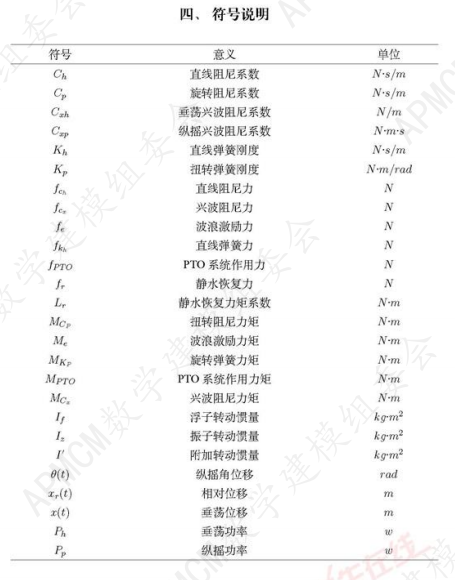
\includegraphics[width=0.65\textwidth]{Figure/符号表.png}\\
		\small 图：本文符号表
	\end{center}
\end{frame}


\section{模型的建立与求解思考}
\begin{frame}
	\frametitle{问题一·建模（1/6）：坐标系与受力分析}
	\scriptsize
	\begin{block}{坐标系的选取}
		\begin{itemize}
			\item 装置在海面做\textbf{六自由度}运动，本题只考虑竖直方向的\textbf{垂荡}（沿 $Z$ 轴）与绕 $Y$ 轴的\textbf{纵摇}
			\item \textbf{大地坐标系} $OXYZ$：原点取静止时浮子的重心，浮子运动时坐标系固定不动
			\item \textbf{固体坐标系} $oxyz$：原点取与静止时振子中心重合的浮子上一点，随浮子运动而移动
			\item 振子相对浮子的位移 $x_r(t)=x_2(t)-x_1(t)$
		\end{itemize}
	\end{block}
	\begin{block}{受力分析（仅垂荡）}
		\begin{itemize}
			\item \textbf{浮子}受：波浪激励力 $f\cos\omega t$、附加惯性力（附加质量 $m_a$）、兴波阻尼力、静水恢复力 $-\rho g A x_1$、PTO 系统作用力
			\item \textbf{振子}受：PTO 系统作用力（弹簧力与阻尼力）
		\end{itemize}
	\end{block}
	\begin{exampleblock}{我的想法}
		建模之前先想清楚坐标系和受力，这步看着笨，其实最关键。我以前总是一上来就写方程，写一半才发现漏了力、或者方向搞反，返工很浪费时间。这次跟着论文一步步来，才明白``先受力分析、再列方程''这个顺序到底省多少事。
	\end{exampleblock}
\end{frame}

\begin{frame}
	\frametitle{问题一·建模（2/6）：垂荡运动方程}
	\scriptsize
	\begin{block}{PTO 系统作用力}
		\begin{itemize}
			\item 直线弹簧力：$f_k=-K\big(x_1(t)-x_2(t)\big)$，与相对位移成正比，$K$ 为弹簧刚度
			\item 直线阻尼力：$f_d=-C\big(\dot x_1(t)-\dot x_2(t)\big)$，与相对速度成正比，$C$ 为阻尼系数
		\end{itemize}
	\end{block}
	\begin{block}{牛顿第二定律列方程}
		浮子：$(m_1+m_a)\ddot x_1(t) = f\cos\omega t + f_d + f_k - \rho g A x_1$\\
		振子：$m_2\ddot x_2(t) = -f_d - f_k$\\
		代入 $f_k,f_d$ 整理后得到关于 $x_1,x_2$ 的\textbf{二元二阶常微分方程组}
	\end{block}
	\begin{exampleblock}{我的想法}
		PTO 的弹簧力和阻尼力写清楚后，两个方程其实是``一条链''：浮子被波浪推着走，振子被浮子带着走。我列方程时犯过错：忘了振子上的力是浮子的反力，方向写反导致结果全不对。后来想明白``作用力与反作用力''，一下子就通了。
	\end{exampleblock}
\end{frame}

\begin{frame}
	\frametitle{问题一·建模（3/6）：四阶龙格库塔求解}
	\scriptsize
	\begin{columns}[T]
		\column{0.55\textwidth}
		\begin{block}{为什么自己改进}
			\begin{itemize}
				\item 要求前 40 周期、0.2s 间隔的位移和速度，MATLAB 自带 ode45 不便精确控制采样
				\item 直接对\textbf{四阶龙格库塔}（截断误差 $O(h^5)$）改进，精度与采样同时满足
			\end{itemize}
		\end{block}
		\begin{block}{二阶转一阶}
			令 $u_1=x_1,\ u_2=\dot x_1,\ v_1=x_2,\ v_2=\dot x_2$，把二元二阶方程组改写为\textbf{一阶四元方程组}
		\end{block}
		\begin{block}{递推公式}
			$y_{n+1}=y_n+\frac{h}{6}(k_1+2k_2+2k_3+k_4)$\\
			$k_1=f(t_n,y_n)$，$k_2=f(t_n+\frac{h}{2},y_n+\frac{h}{2}k_1)$\\
			$k_3=f(t_n+\frac{h}{2},y_n+\frac{h}{2}k_2)$，$k_4=f(t_n+h,y_n+hk_3)$
		\end{block}
		\column{0.45\textwidth}
		\begin{block}{参数与初值}
			\begin{itemize}
				\item 步长 $h=10^{-4}$，递推长度 40 个波浪周期
				\item 初值（静水平衡）：$x_1(0)=x_2(0)=0$，$\dot x_1(0)=\dot x_2(0)=0$
				\item 按 0.2s 间隔采样，保存结果
			\end{itemize}
		\end{block}
		\begin{center}
			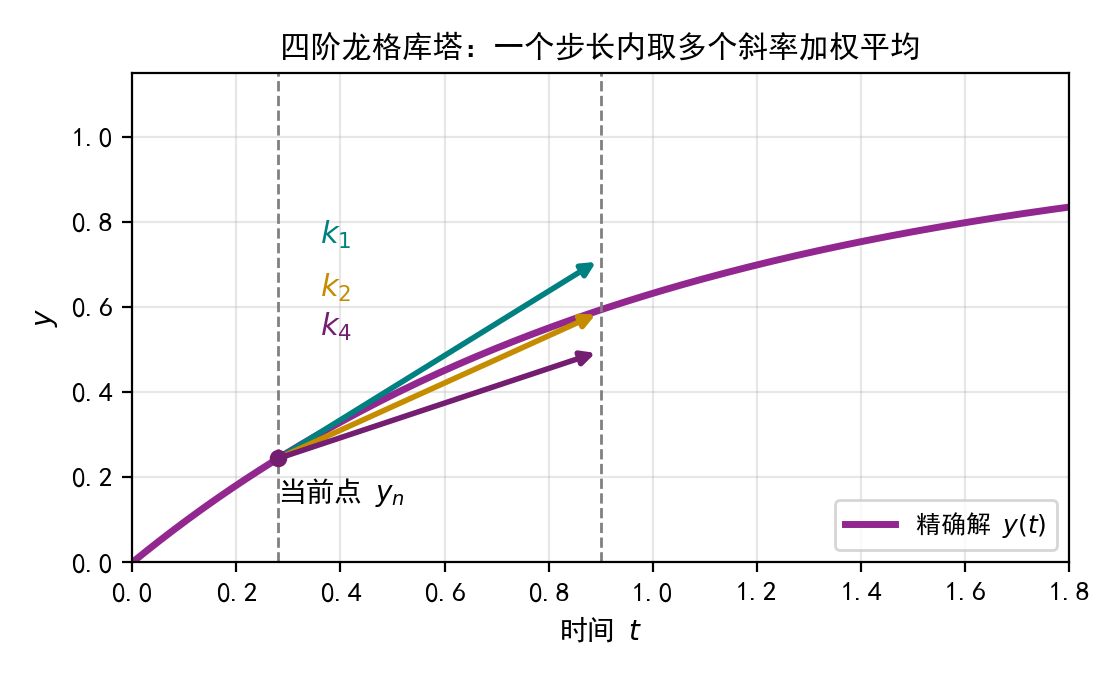
\includegraphics[height=0.14\textheight]{Figure/fig_rk4.png}\\
			\scriptsize 四阶龙格库塔：一个步长内取多个斜率加权（示意）
		\end{center}
		\begin{exampleblock}{我的想法}
			二阶转一阶是标准动作，但我以前只停留在``会用''，没想过步长为什么要取这么小。自己跑一次才发现：步长一大，40 个周期算到后面就抖得没法看，$h=10^{-4}$ 才稳得下来。
		\end{exampleblock}
	\end{columns}
\end{frame}

\begin{frame}
	\frametitle{问题一·结果（1/3）：大地坐标系下的运动（题 1.(1)）}
	\scriptsize
	\begin{columns}[c]
		\column{0.55\textwidth}
		\begin{center}
			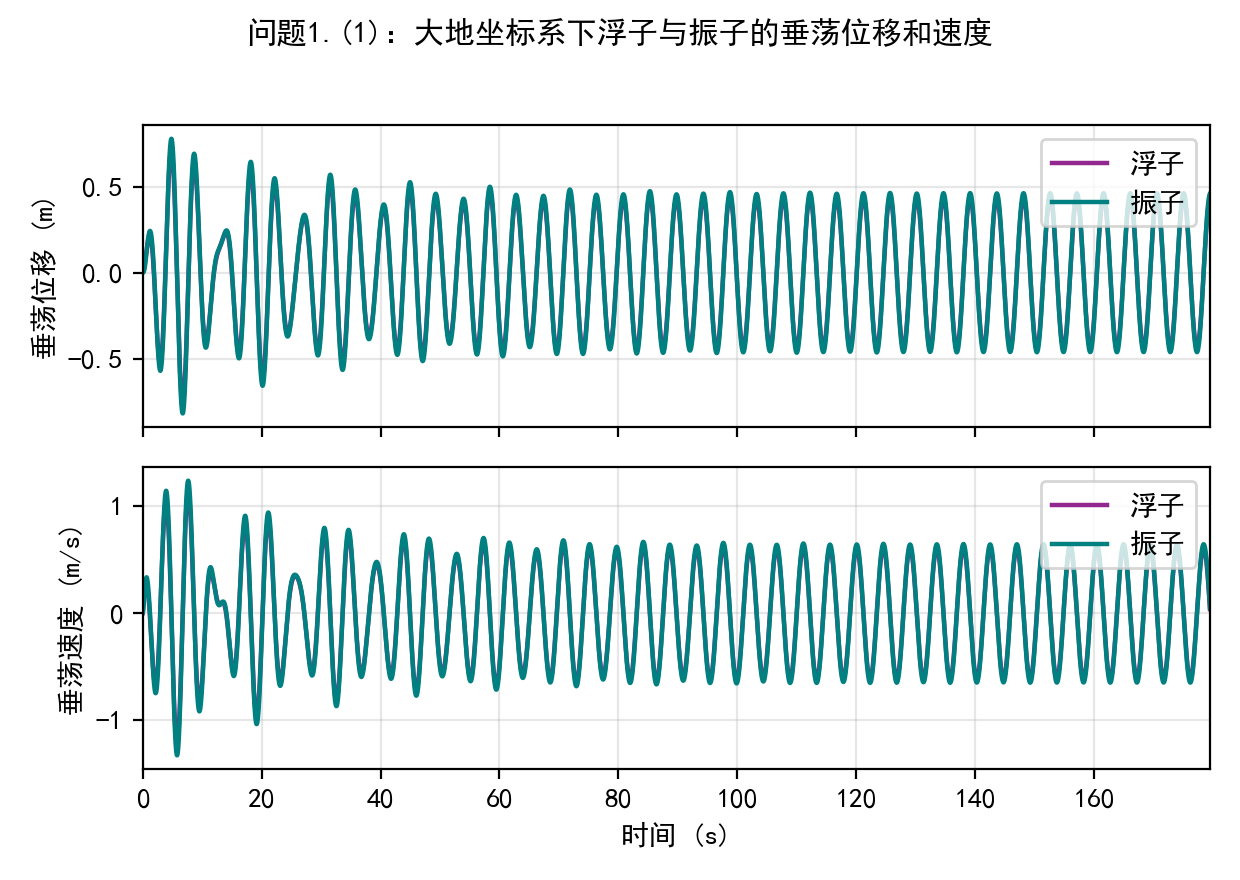
\includegraphics[width=\textwidth]{Figure/fig_sim_01.png}
		\end{center}
		\column{0.45\textwidth}
		\begin{exampleblock}{我的想法}
			第一眼看到浮子和振子的位移、速度曲线，我有点意外——两条线几乎贴在一起。这说明绝对运动里看不出振子相对浮子在干什么，也提醒我：看图不能只看表面，得想清楚``什么量才是我们真正关心的''。
		\end{exampleblock}
	\end{columns}
\end{frame}

\begin{frame}
	\frametitle{问题一·结果（2/3）：相对位移下的运动（题 1.(1)）}
	\scriptsize
	\begin{columns}[c]
		\column{0.55\textwidth}
		\begin{center}
			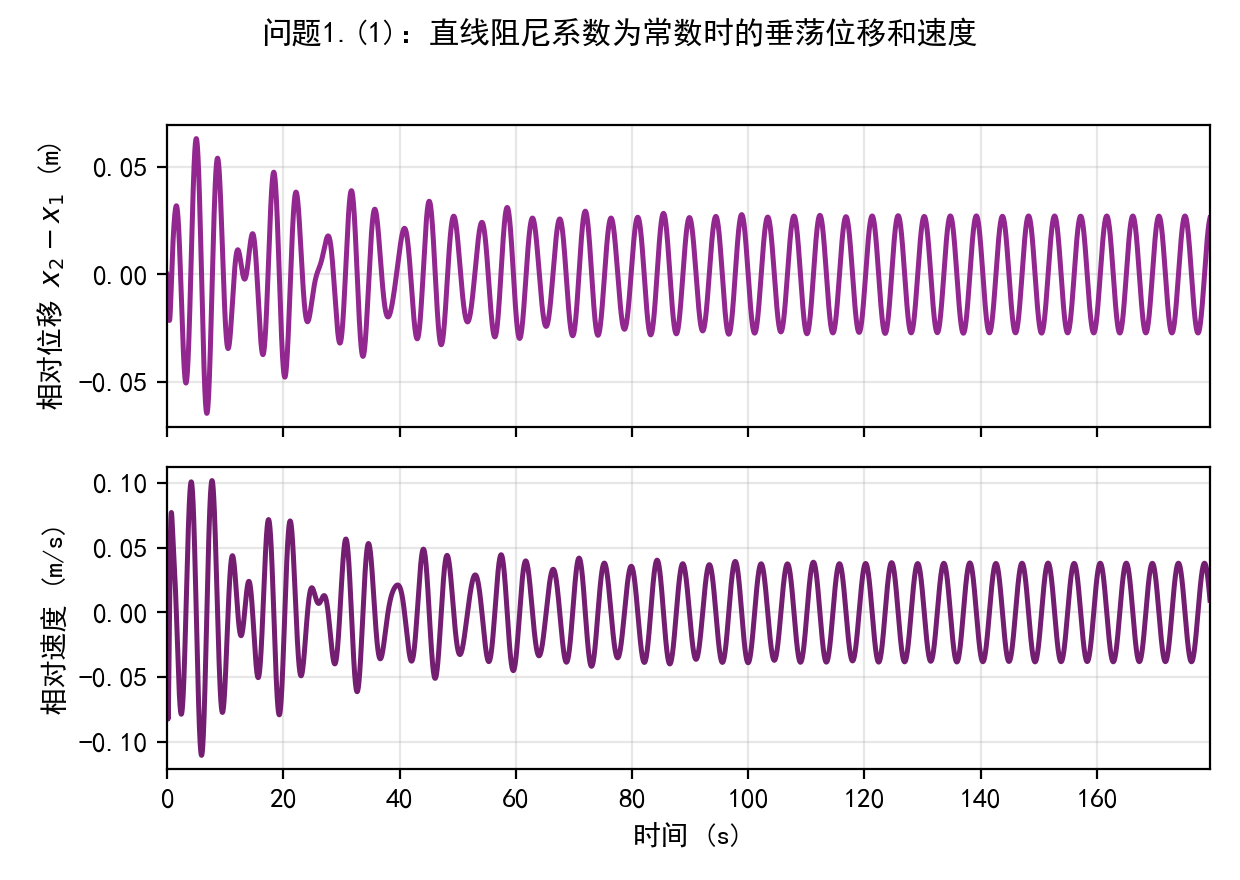
\includegraphics[width=\textwidth]{Figure/fig_sim_02.png}
		\end{center}
		\column{0.45\textwidth}
		\begin{exampleblock}{我的想法}
			把坐标换成振子相对浮子的位移和速度，相对运动立刻清楚了。相对速度大，阻尼器做功就大，PTO 才有能量输出。``换个参考系看数据''这个小技巧，我这次是实打实学会了。
		\end{exampleblock}
	\end{columns}
\end{frame}

\begin{frame}
	\frametitle{问题一·结果（3/3）：变阻尼下的运动（题 1.(2)）}
	\scriptsize
	\begin{columns}[c]
		\column{0.55\textwidth}
		\begin{center}
			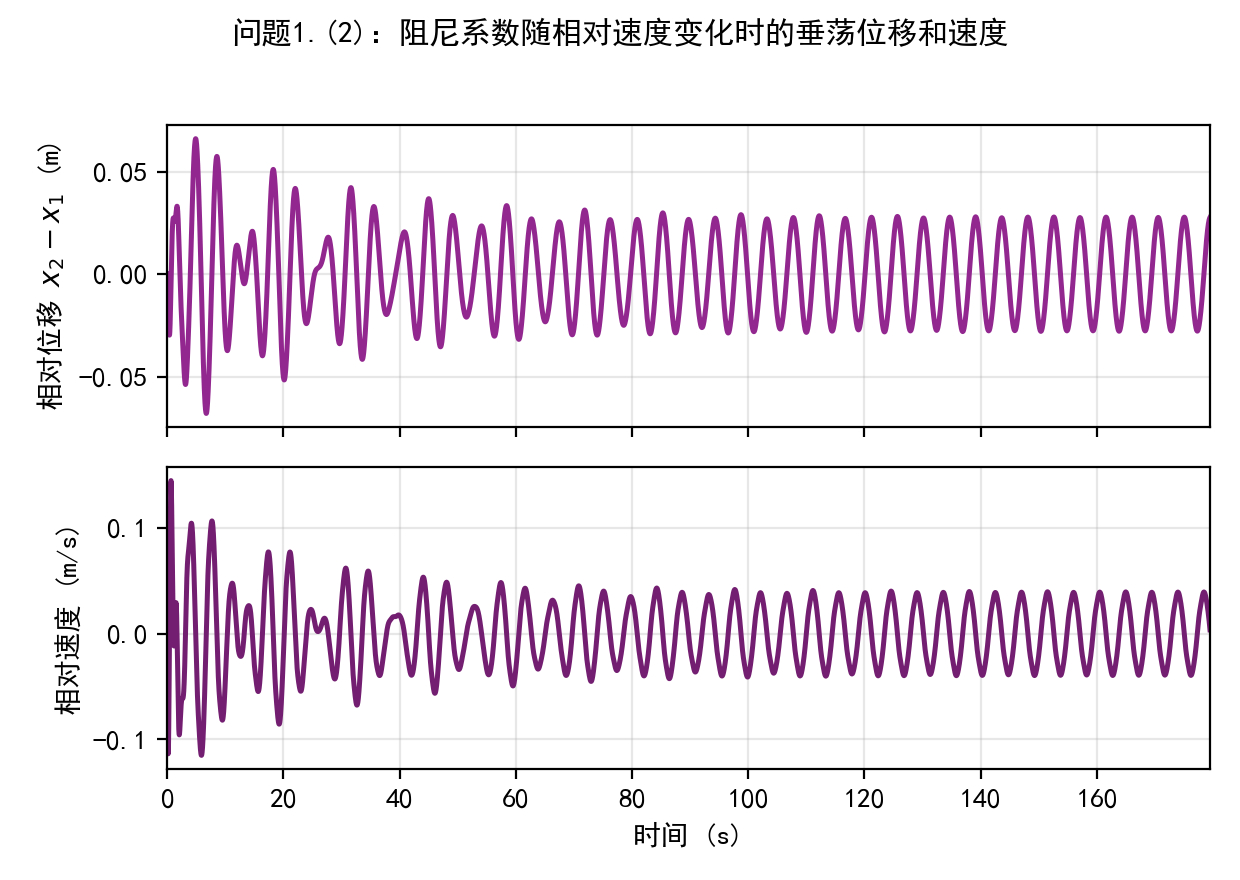
\includegraphics[width=\textwidth]{Figure/fig_sim_03.png}
		\end{center}
		\column{0.45\textwidth}
		\begin{exampleblock}{我的想法}
			变阻尼（$C=10000\,|v_r|^{0.5}$）和常数阻尼比，相对运动的形态明显不同。我这才体会到：阻尼模型不是随便选的，它直接决定运动结果。题目特意把两种情况分开让我们算，大概就是这个用意。
		\end{exampleblock}
	\end{columns}
\end{frame}

\begin{frame}
	\frametitle{问题二·建模（1/6）：平均功率函数}
	\scriptsize
	\begin{block}{瞬时功率}
		平动功率 $P=F\cdot v$，PTO 直线阻尼器消耗的瞬时功率为
		\begin{center}
			$P(t)=C\big(\dot x_1(t)-\dot x_2(t)\big)^2$
		\end{center}
	\end{block}
	\begin{block}{平均功率}
		取系统振动\textbf{稳态响应后}的一段时间 $[t_1,t_2]$ 求平均：
		\begin{center}
			$P_{avg}=\dfrac{1}{t_2-t_1}\int_{t_1}^{t_2} C\,(\dot x_1-\dot x_2)^2\,dt$
		\end{center}
		$C\in[0,100000]$；题 1.(1) 中 $C$ 为常量，题 1.(2) 中 $C=\alpha\,|v_r|^{\beta}$
	\end{block}
	\begin{exampleblock}{我的想法}
		平均功率的定义看着简单，但有个细节我一开始没注意：为什么只取稳态段求平均？因为前面有一段瞬态，功率不稳定，取平均会把结果带偏。我自己画出功率曲线才真正理解这个取舍。
	\end{exampleblock}
\end{frame}

\begin{frame}
	\frametitle{问题二·建模（2/6）：优化模型建立}
	\scriptsize
	\begin{block}{目标函数}
		$\max\limits_{C}\ P_{avg}(C)$，其中 $P_{avg}=\dfrac{1}{t_2-t_1}\displaystyle\int_{t_1}^{t_2} C\big(\dot x_1-\dot x_2\big)^2\,dt$
	\end{block}
	\begin{block}{约束条件}
		\begin{itemize}
			\item \textbf{运动方程约束}：垂荡运动模型（问题一的方程组）
			\item \textbf{情况 (1)}：$C$ 为常量，$C\in[0,100000]$
			\item \textbf{情况 (2)}：$C=\alpha\,|v_r|^{\beta}$，$\alpha\in[0,100000]$，$\beta\in[0.1,1]$
			\item 波浪激励 $f\cos\omega t$，初值取静水平衡
		\end{itemize}
	\end{block}
	\begin{exampleblock}{我的想法}
		把工程问题写成``目标 + 决策量 + 约束''的优化模型，是数模里最常用的套路。这里两种情况的范围都列全了，照着就能算。我学到的经验：约束写得越具体，求解越省事，也越能说服评委。
	\end{exampleblock}
\end{frame}

\begin{frame}
	\frametitle{问题二·建模（3/6）：数值求解——梯形法}
	\scriptsize
	\begin{columns}[T]
		\column{0.5\textwidth}
		\begin{block}{功率积分离散化}
			\begin{itemize}
				\item 用\textbf{梯形法}求积分：步长足够小时，把连续函数用梯形面积之和近似
				\item 时间步长取 $10^{-4}$，满足精度要求
				\item 因前期位移不稳定，截取稳态段 $[100,180]$s 求平均功率
			\end{itemize}
		\end{block}
		\begin{block}{先粗后精的寻优}
			\begin{itemize}
				\item \textbf{粗略寻优}：增大阻尼系数遍历步长，得到功率随阻尼系数的分布
				\item \textbf{遗传算法精求}：避免局部最优、并行搜索、按概率选最优，迭代 200 次
			\end{itemize}
		\end{block}
		\column{0.5\textwidth}
		\begin{center}
			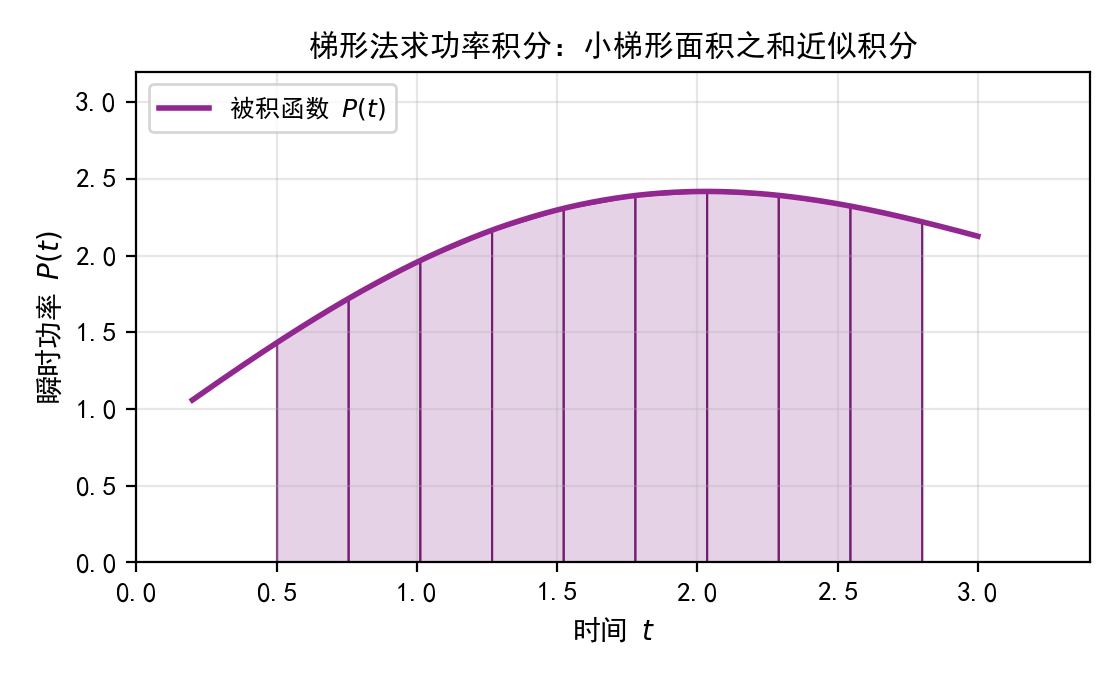
\includegraphics[height=0.3\textheight]{Figure/fig_sim_04.png}
		\end{center}
		\begin{exampleblock}{我的想法}
			梯形法是我这次重点学的对象：积分不会算没关系，用一堆小梯形去近似，步长越小越接近真值。更妙的是``先粗扫、再遗传算法精找''的组合，直接暴力遍历太慢，遗传算法又能跳出局部最优。这个思路我记下了，以后做优化题都能用。
		\end{exampleblock}
	\end{columns}
\end{frame}

\begin{frame}
	\frametitle{问题二·结果（1/2）：题 2.(1) 常数阻尼}
	\scriptsize
	\begin{columns}[c]
		\column{0.55\textwidth}
		\begin{center}
			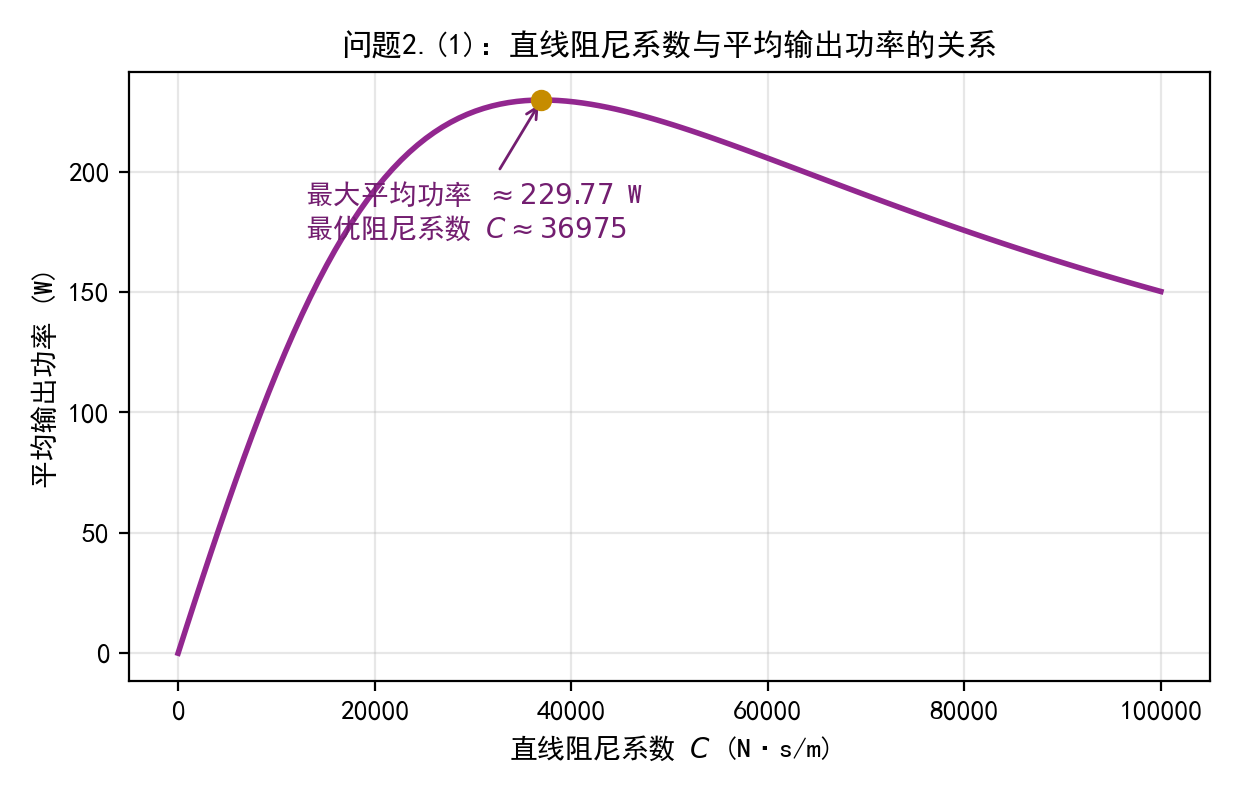
\includegraphics[width=\textwidth]{Figure/fig_sim_05.png}
		\end{center}
		\column{0.45\textwidth}
		\begin{exampleblock}{我的想法}
			扫完阻尼系数画出功率曲线，看到单峰的那一刻我是服气的：阻尼太小耗能不足，太大又把运动锁死，中间必然有个最好的值。我复现出 $C\approx37186$、$P\approx229.77$W，和论文的 37639、229.68W 基本一致，说明模型没建错，心里踏实了不少。
		\end{exampleblock}
	\end{columns}
\end{frame}

\begin{frame}
	\frametitle{问题二·结果（2/2）：题 2.(2) 阻尼与幂指数（三维）}
	\scriptsize
	\begin{columns}[c]
		\column{0.55\textwidth}
		\begin{center}
			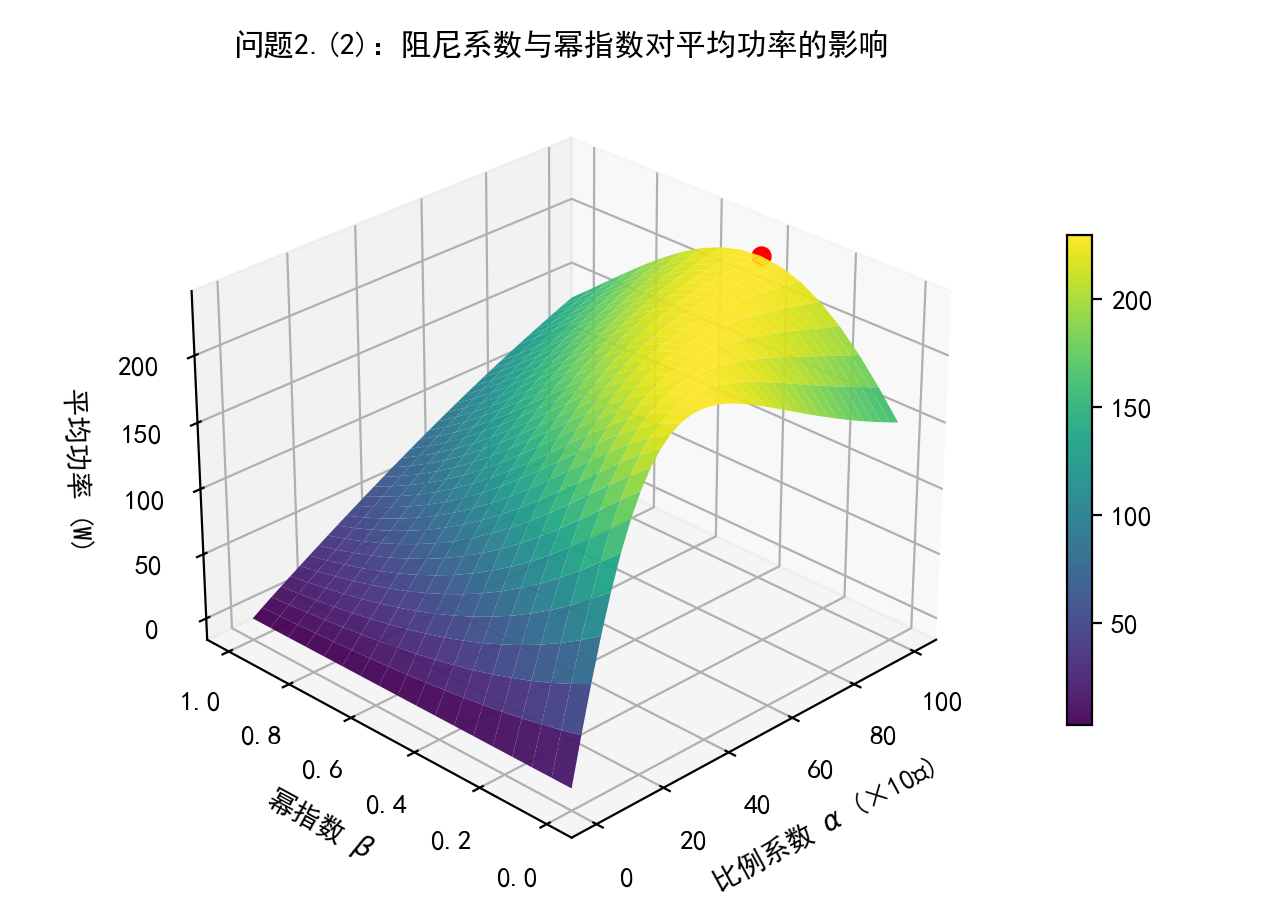
\includegraphics[width=\textwidth]{Figure/fig_sim_06.png}
		\end{center}
		\column{0.45\textwidth}
		\begin{exampleblock}{我的想法}
			问题 2.(2) 要同时定 $\alpha$ 和 $\beta$，是一张三维面。把面画出来我才意识到：两个参数是``一起''影响功率的，不能拆开各自求最优。我复现的峰位和论文有点出入，但``存在最优区域''这个整体结论是一致的。
		\end{exampleblock}
	\end{columns}
\end{frame}

\begin{frame}
	\frametitle{问题三·建模（1/4）：转动惯量计算}
	\scriptsize
	\begin{block}{先定转轴、再求重心}
		\begin{itemize}
			\item 纵摇时物体绕 $y$ 轴近似\textbf{穿过重心}，因此先确定浮子重心位置
			\item 浮子外壳看作\textbf{圆面 + 圆柱侧面 + 圆锥侧面}的组合体，重心用组合体重心公式 $\bar z=\dfrac{\sum m_i z_i}{\sum m_i}$
		\end{itemize}
	\end{block}
	\begin{block}{平行移轴与垂直轴定理}
		\begin{itemize}
			\item \textbf{平行移轴定理}：$I=I_C+md^2$（$d$ 为平行轴到质心轴距离）
			\item \textbf{垂直轴定理}：薄片对垂直轴惯量 $=$ 平面内两正交轴惯量之和
			\item 得浮子 $I_1=58289.43\,\mathrm{kg\cdot m^2}$；振子惯量随相对位移变化 $I_2=202.75+243.3\,(0.8+x_r(t))^2$
		\end{itemize}
	\end{block}
	\begin{exampleblock}{我的想法}
		问题三多了纵摇，第一步居然是算转动惯量。平行移轴、垂直轴定理我上课学过但从没用过，这次才发现它们是``组合体''求惯量的标准工具。坦白讲这一页我是对着课本啃下来的。
		\end{exampleblock}
\end{frame}

\begin{frame}
	\frametitle{问题三·建模（2/4）：纵摇运动方程}
	\scriptsize
	\begin{block}{受力分析与 PTO 力矩}
		\begin{itemize}
			\item \textbf{浮子}受：波浪激励力矩 $L\cos\omega t$、附加惯性力矩、兴波阻尼力矩、静水恢复力矩 $M_s=-L_s\theta_1$、PTO 作用力矩；\textbf{振子}只受 PTO 作用力矩
			\item 旋转弹簧力矩：$M_k=-K_t\big(\theta_1(t)-\theta_2(t)\big)$
			\item 扭转阻尼力矩：$M_d=-C_t\big(\dot\theta_1(t)-\dot\theta_2(t)\big)$
		\end{itemize}
	\end{block}
	\begin{block}{牛顿第二定律（转动）}
		浮子：$(I_1+I_a)\ddot\theta_1 = L\cos\omega t + M_k + M_d - L_s\theta_1$\\
		振子：$I_2\ddot\theta_2 = -M_k - M_d$\\
		与问题一垂荡方程\textbf{联立} $\Rightarrow$ \textbf{四元二阶微分方程组}
	\end{block}
	\begin{exampleblock}{我的想法}
		纵摇和垂荡其实是同一个套路换个自由度，方程结构几乎一样。联立后从二元变四元，量变多但不算难。我体会到：多自由度问题往往是``单自由度的复制加耦合''，会一个就会一串。
	\end{exampleblock}
\end{frame}

\begin{frame}
	\frametitle{问题三·建模（3/4）：求解}
	\scriptsize
	\begin{block}{转一阶多元方程组}
		\begin{itemize}
			\item 把垂荡 + 纵摇的四元二阶方程组改写为\textbf{一阶八元方程组}
			\item 初值（静水平衡）：各（角）位移、速度、角速度均为 0
		\end{itemize}
	\end{block}
	\begin{block}{龙格库塔递推}
		\begin{itemize}
			\item 与问题一同法，用\textbf{四阶龙格库塔}递推（步长 $10^{-4}$）
			\item 递推前 40 个波浪周期，按 0.2s 间隔采样
			\item 输出浮子、振子的\textbf{位移、速度、角位移、角速度}四组量
		\end{itemize}
	\end{block}
	\begin{exampleblock}{我的想法}
		求解流程和问题一一模一样，只是状态量从 4 个变成 8 个。这套``转一阶 + 龙格库塔''的方法从问题一用到问题四，一路没换过。我最大的收获是：方法不怕少，用熟一套就够应对很多题。
	\end{exampleblock}
\end{frame}

\begin{frame}
	\frametitle{问题三·结果：前 40 周期垂荡与纵摇运动}
	\scriptsize
	\begin{columns}[c]
		\column{0.55\textwidth}
		\begin{center}
			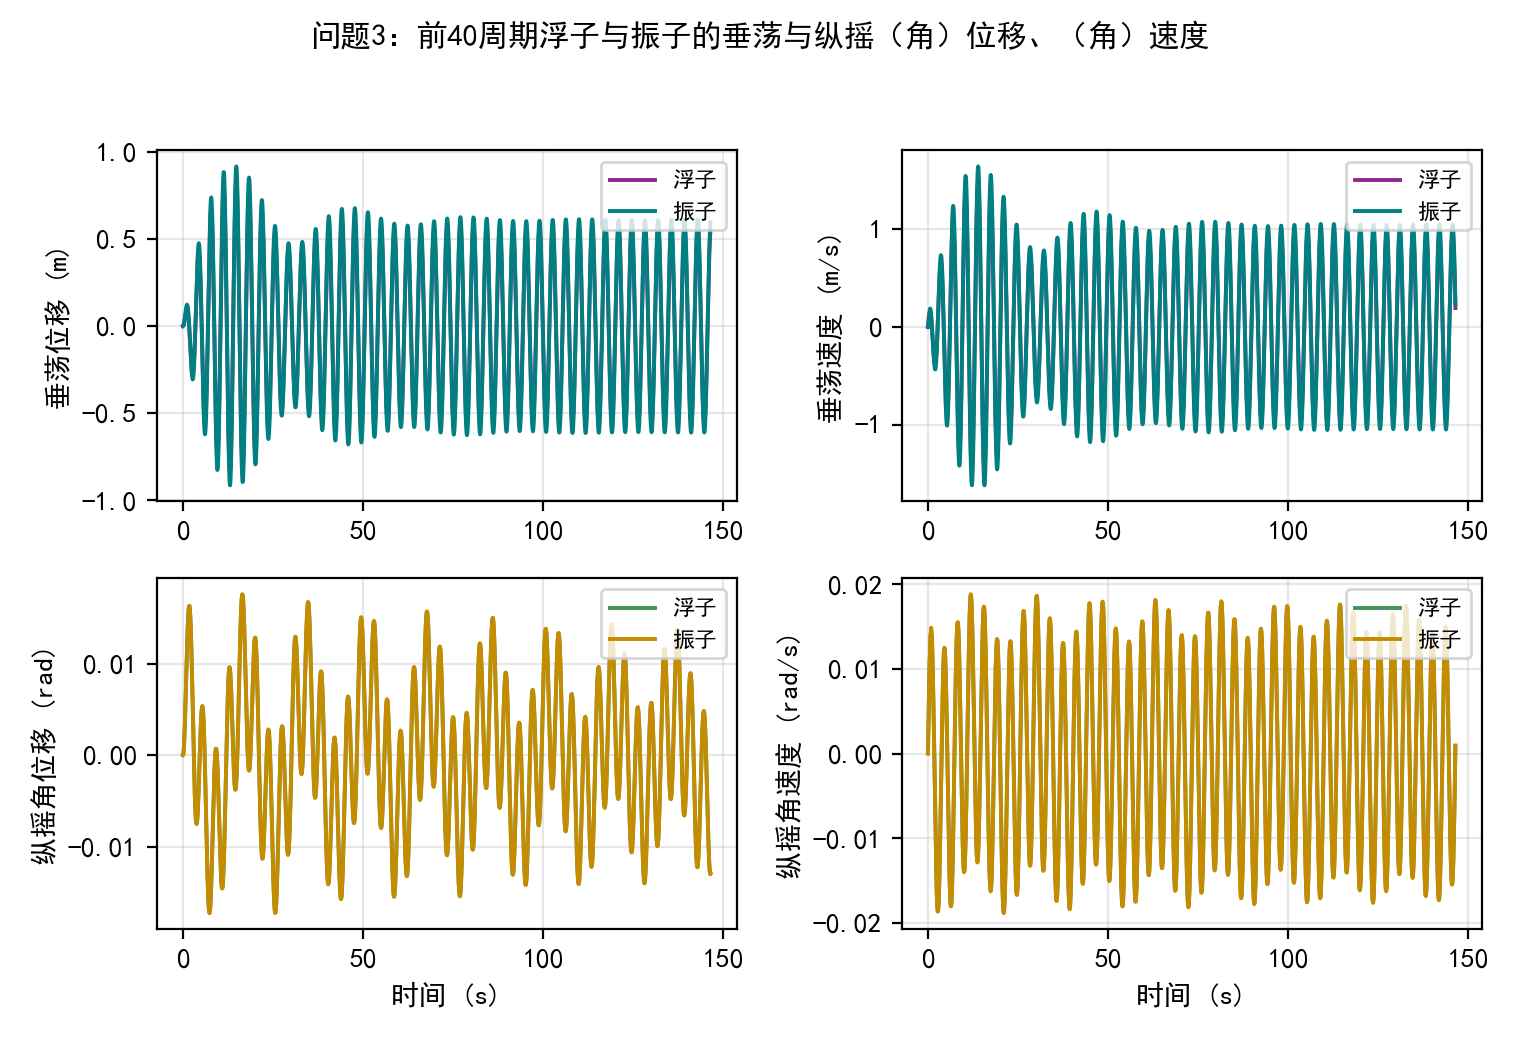
\includegraphics[width=\textwidth]{Figure/fig_sim_07.png}
		\end{center}
		\column{0.45\textwidth}
		\begin{exampleblock}{我的想法}
			四张子图把垂荡和纵摇都画出来了。最让我意外的是纵摇角只有 0.018 rad 左右，特别小。这正好解释了后面问题四里``旋转阻尼几乎不影响功率''——纵摇本身动得就少，旋转阻尼自然使不上劲。作者前后呼应的逻辑，我这次是看懂了。
		\end{exampleblock}
	\end{columns}
\end{frame}

\begin{frame}
	\frametitle{问题四·建模（1/3）：功率函数推导}
	\scriptsize
	\begin{block}{瞬时功率}
		转动功率 $P=M\cdot\omega$；PTO 总瞬时功率 = 直线阻尼功率 + 旋转阻尼功率
		\begin{center}
			$P(t)=C\big(\dot x_1-\dot x_2\big)^2 + C_t\big(\dot\theta_1-\dot\theta_2\big)^2$
		\end{center}
	\end{block}
	\begin{block}{平均功率}
		取稳态响应后的一段时间 $[t_1,t_2]$ 求平均：
		\begin{center}
			$P_{avg}=\dfrac{1}{t_2-t_1}\displaystyle\int_{t_1}^{t_2}\Big[C\big(\dot x_1-\dot x_2\big)^2 + C_t\big(\dot\theta_1-\dot\theta_2\big)^2\Big]dt$
		\end{center}
	\end{block}
	\begin{exampleblock}{我的想法}
		问题四的功率就是问题二加了一项旋转项，公式完全继承。这种``前问为后问做铺垫''的写法，让读者不用重复理解新概念。我要学的就是这种递进式的组织方式。
	\end{exampleblock}
\end{frame}

\begin{frame}
	\frametitle{问题四·建模（2/3）：优化模型建立}
	\scriptsize
	\begin{block}{目标函数}
		\begin{center}
			$\max\limits_{C,\,C_t}\ P_{avg}(C,C_t)$
		\end{center}
	\end{block}
	\begin{block}{约束条件}
		\begin{itemize}
			\item \textbf{运动方程约束}：垂荡 + 纵摇联立的四元二阶方程组
			\item 直线阻尼系数 $C\in[0,100000]$，旋转阻尼系数 $C_t\in[0,100000]$
			\item 波浪频率 $\omega=1.9806\,\mathrm{s^{-1}}$；初值取静水平衡
		\end{itemize}
	\end{block}
	\begin{exampleblock}{我的想法}
		目标、决策量、约束三件套又来一遍，只是决策量从问题二的一个变成两个（$C$ 和 $C_t$），求解框架完全相同。看懂问题二，问题四的模型基本就懂了一半。我意识到：赛题的四问通常一步步升级，前一问的成果后一问直接复用。
	\end{exampleblock}
\end{frame}

\begin{frame}
	\frametitle{问题四·结果：双阻尼系数下的功率分布（三维）}
	\scriptsize
	\begin{columns}[c]
		\column{0.55\textwidth}
		\begin{center}
			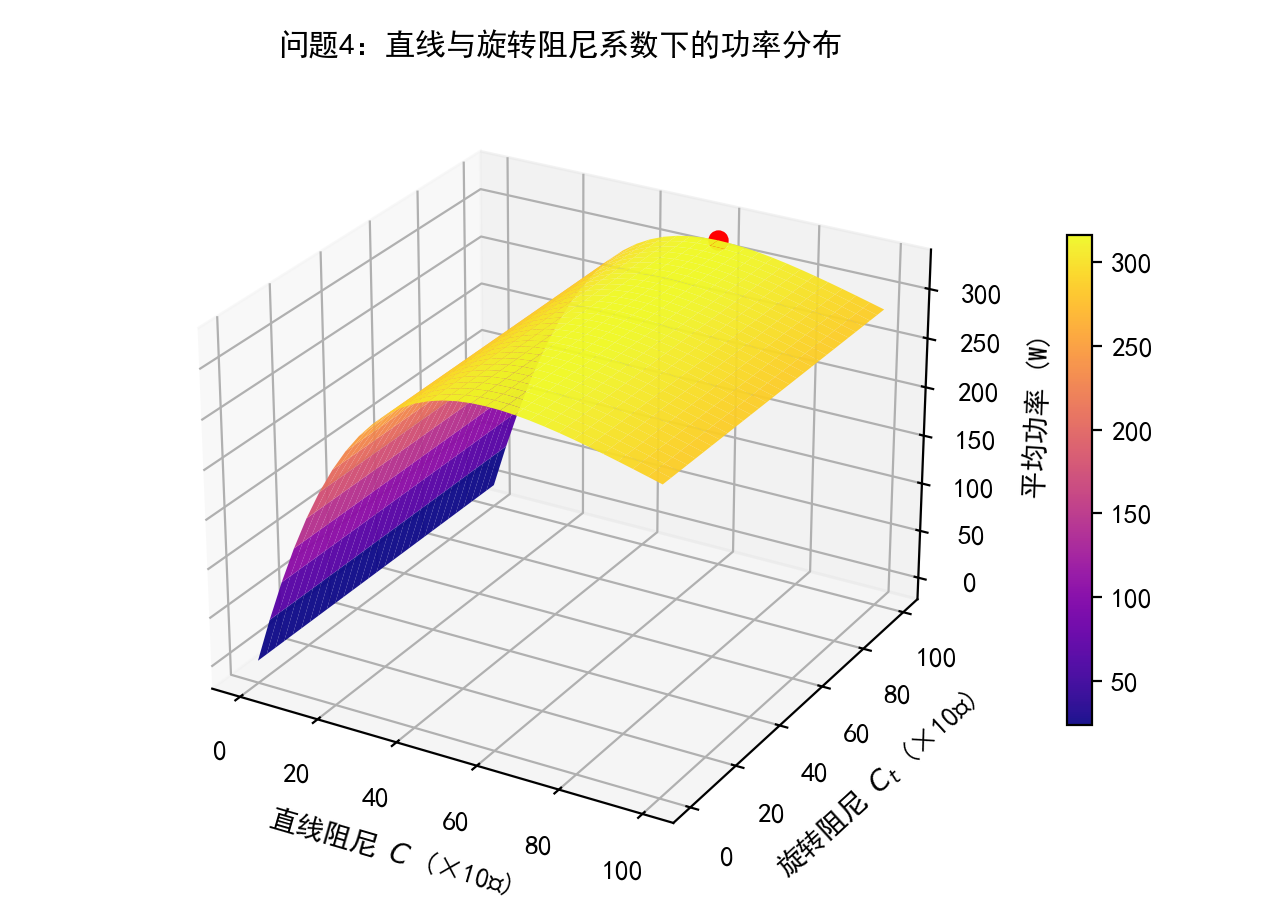
\includegraphics[width=\textwidth]{Figure/fig_sim_08.png}
		\end{center}
		\column{0.45\textwidth}
		\begin{exampleblock}{我的想法}
			双阻尼的功率分布面最有意思的是：沿旋转阻尼方向几乎一马平川，沿直线阻尼方向才有峰值。这说明参数分``敏感''和``不敏感''，优化时抓大放小就行。我复现的最优功率 316.50W 和论文的 316.58W 也很接近。
		\end{exampleblock}
	\end{columns}
\end{frame}

\section{模型检验（分析）思考}
\begin{frame}
	\frametitle{模型检验（一）：检验原理与垂荡检验}
	\scriptsize
	\begin{columns}[T]
		\column{0.55\textwidth}
		\begin{block}{检验原理}
			\begin{itemize}
				\item 装置属\textbf{简谐激励下线性系统的受迫振动}，稳定后振动周期应与波浪激励周期接近
				\item 比较实际响应周期与理论激励周期的方差 $\delta$，$\delta$ 小则模型正确
			\end{itemize}
		\end{block}
		\begin{block}{垂荡模型检验结果}
			\begin{itemize}
				\item 题 1.(1)：$\delta=0.0017<0.1\%$
				\item 题 1.(2)：$\delta=0.0034<0.4\%$
			\end{itemize}
		\end{block}
		\column{0.45\textwidth}
		\begin{center}
			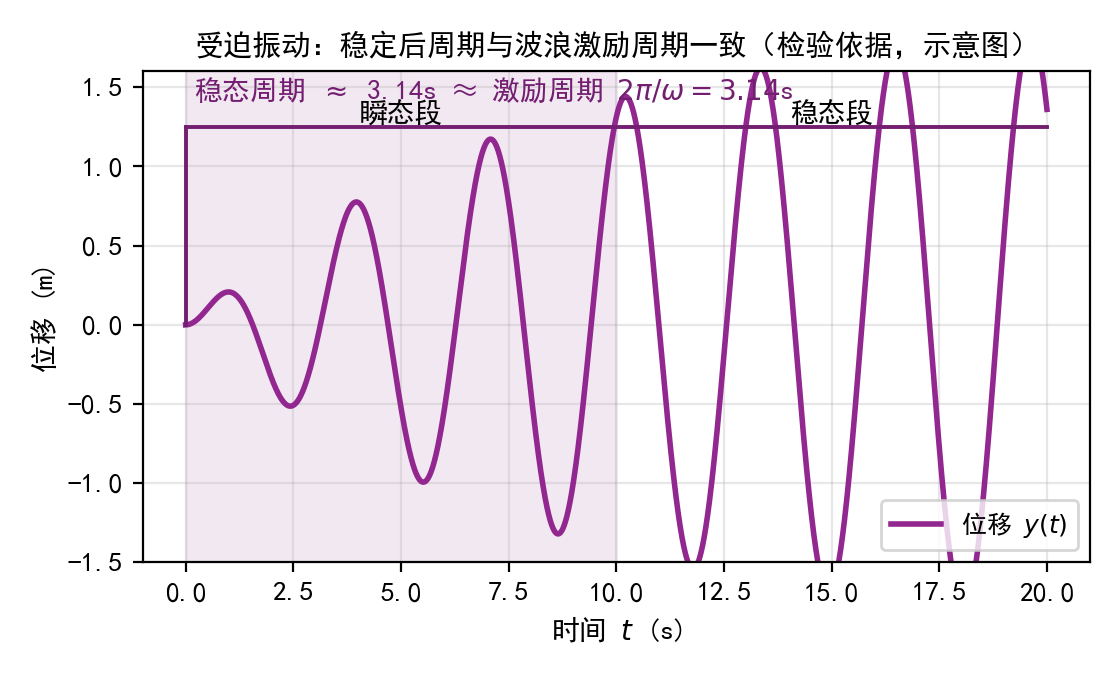
\includegraphics[height=0.24\textheight]{Figure/fig_forced.png}\\
			\scriptsize 受迫振动稳态周期约等于激励周期（示意）
		\end{center}
		\begin{exampleblock}{我的想法}
			我以前以为检验就必须有实验数据，看了这篇才明白：没有实验也能验——用物理常识。受迫振动稳定后周期必须等于激励周期，这是硬道理，拿它一对就知道模型对不对。``用常识当标尺''这个思路很受用。
		\end{exampleblock}
	\end{columns}
\end{frame}

\begin{frame}
	\frametitle{模型检验（二）：纵摇检验与可靠性检验}
	\scriptsize
	\begin{columns}[T]
		\column{0.55\textwidth}
		\begin{block}{纵摇模型检验结果}
			题 3：$\delta=0.00036<0.04\%$，方差极小，认为模型正确
		\end{block}
		\begin{block}{结果可靠性检验}
			\begin{itemize}
				\item 问题三要算浮子转动惯量，可能引入误差
				\item 对问题三参数加 $\pm 1\%$ 扰动，比较扰动前后输出偏差
				\item 偏差 $<0.10\%$，结果对参数不敏感，求解可靠
			\end{itemize}
		\end{block}
		\column{0.45\textwidth}
		\begin{center}
			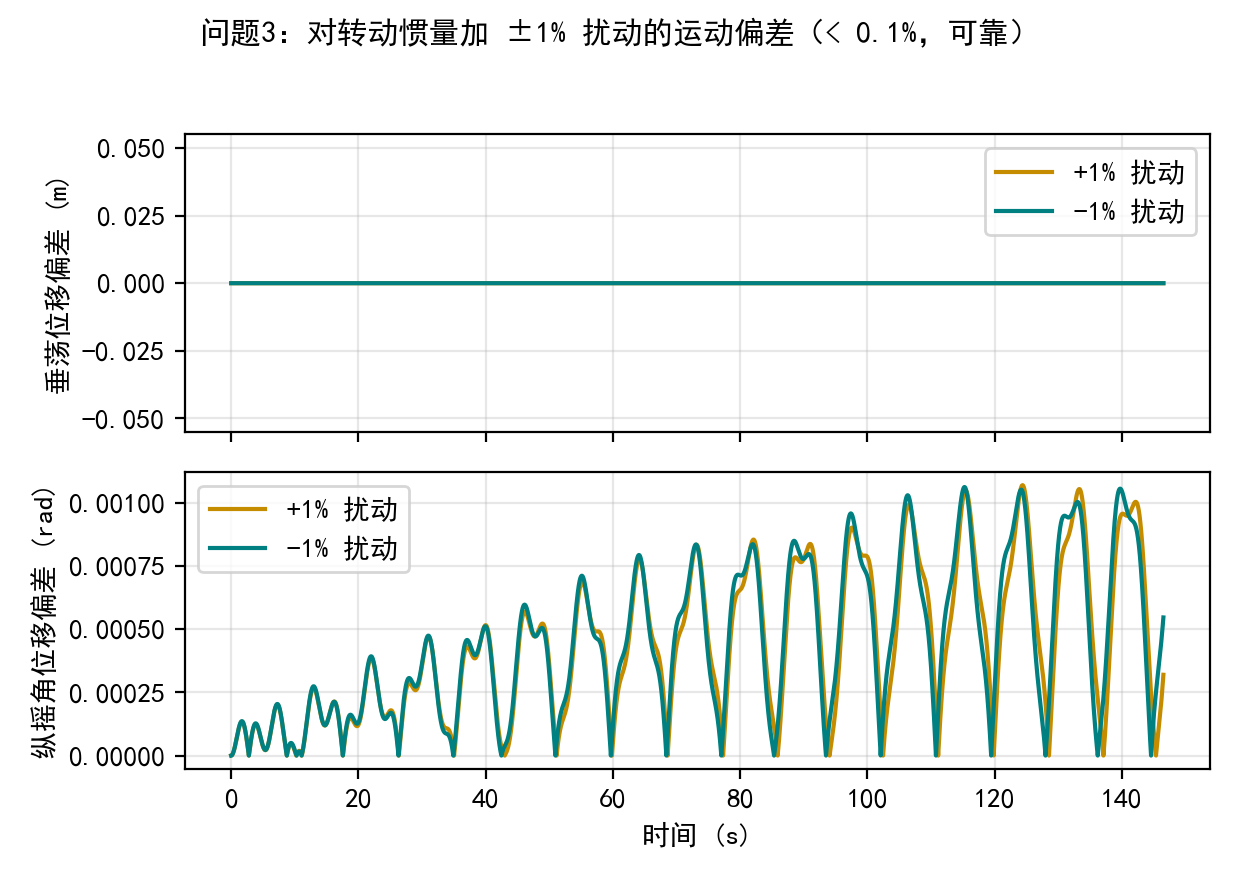
\includegraphics[height=0.24\textheight]{Figure/fig_sim_09.png}\\
			\scriptsize 对转动惯量加 $\pm1\%$ 扰动后的运动偏差
		\end{center}
		\begin{exampleblock}{我的想法}
			我亲手把转动惯量加了 $\pm1\%$ 再重算，偏差确实很小。之前总觉得``检验''是走流程，这次自己动手才懂：模型对参数不敏感，结果才值得相信。这个``扰动检验''我以后写论文也要用。
		\end{exampleblock}
	\end{columns}
\end{frame}

\begin{frame}
	\frametitle{模型检验（三）：小结}
	\scriptsize
	\begin{block}{检验做对了什么}
		\begin{itemize}
			\item 检验标准可验证：用物理常识（周期吻合），不是自说自话
			\item 既验\textbf{模型方程}的正确性（周期方差），又验\textbf{求解结果}的可靠性（参数扰动）
			\item 全部给出量化阈值（0.1\%、0.4\%、0.04\%、0.10\%），说服力强
		\end{itemize}
	\end{block}
	\begin{exampleblock}{我的想法}
		检验部分篇幅不长，但``验什么、怎么验、阈值多少''都交代清楚。让我自己写，可能就一句``误差很小''。从这篇里我学到：检验要和物理常识挂钩，数字要给具体阈值，才站得住脚。
	\end{exampleblock}
\end{frame}

\section{总结}
\begin{frame}
	\frametitle{总结（一）：模型优点}
	\scriptsize
	\begin{block}{优点}
		\begin{enumerate}
			\item \textbf{建模有依据}：基于牛顿第二定律做受力分析，数值解较符合实际
			\item \textbf{计算降难度}：对目标函数做离散化处理（梯形面积近似）
			\item \textbf{算法精度高}：改进四阶龙格库塔 + 遗传算法，实现高精度求解
		\end{enumerate}
	\end{block}
	\begin{exampleblock}{我的收获}
		读完整篇，我最想学的是这三点：建模有受力分析支撑、计算有离散化兜底、求解有先进算法加持。我不一定都能做到，但至少知道了``好论文的建模长什么样''，照着学总不会错。
	\end{exampleblock}
\end{frame}

\begin{frame}
	\frametitle{总结（二）：模型缺点}
	\scriptsize
	\begin{block}{缺点}
		\begin{enumerate}
			\item \textbf{重心计算有简化}：计算浮子重心时忽略浮子厚度等，可能产生偏差
			\item \textbf{忽略耦合效应}：忽略纵摇与垂荡的耦合，对静水恢复力做了简化；实际运动中两自由度会相互影响
		\end{enumerate}
	\end{block}
	\begin{exampleblock}{我的思考}
		作者肯承认自己忽略耦合、简化重心，反而显得可信。我以前以为写缺点会减分，现在觉得：能把缺点说清楚，说明对自己的模型有清醒的认识，这本身就是加分项。这点对我的启发很大。
	\end{exampleblock}
\end{frame}

\begin{frame}
	\frametitle{总结（三）：模型推广与改进}
	\scriptsize
	\begin{block}{推广}
		\begin{itemize}
			\item 方法可用于其他受波浪激励物体的运动分析，可用遗传算法设计最优阻尼系数，对实际生产有借鉴意义
		\end{itemize}
	\end{block}
	\begin{block}{改进方向}
		\begin{itemize}
			\item 实际运动中不同自由度会互相耦合，后续可建立\textbf{纵摇-垂荡耦合运动模型}
		\end{itemize}
	\end{block}
	\begin{exampleblock}{我的想法}
		收尾处说以后要建纵摇-垂荡耦合模型，既是诚实的自我批评，也指明了下一步。我学到的写法是：总结别只复述做完了什么，要落到``以后还能怎么做''。这样的总结才有信息量。
	\end{exampleblock}
\end{frame}
% ---------- 结束页 ----------
\begin{frame}
	\centering
	\Huge{感谢聆听！}\\[1cm]
	\Large{敬请各位老师、同学批评指正}
\end{frame}

\end{document}
